\documentclass[border=10pt]{standalone}
\usepackage{pgfplots}
\pgfplotsset{compat=1.18}
\usepgfplotslibrary{colormaps}

\begin{document}
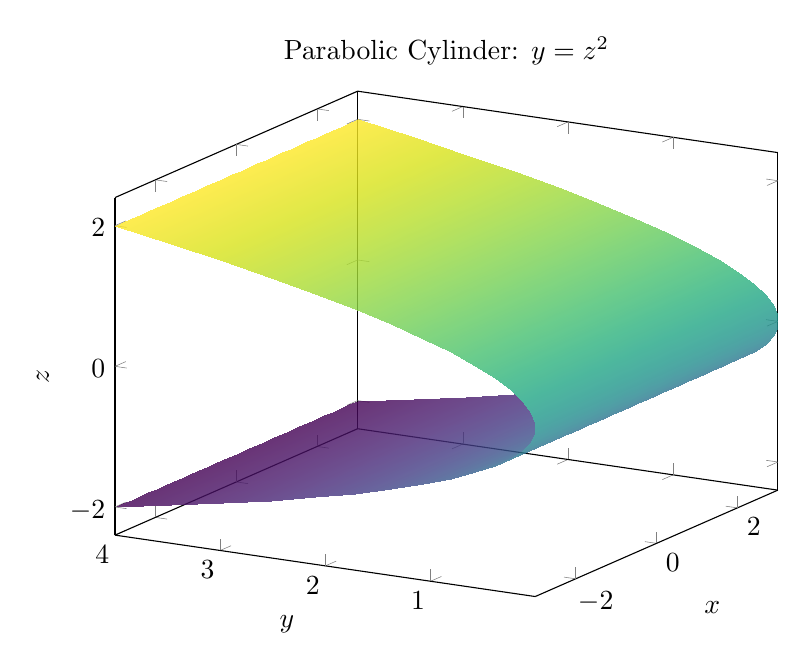
\begin{tikzpicture}
\begin{axis}[
    width=10cm,
    height=8cm,
    xlabel=$x$,
    ylabel=$y$,
    zlabel=$z$,
    title={Parabolic Cylinder: $y = z^2$},
    view={-60}{20},
    colormap/viridis,
    grid=none,
    samples=30,
    domain=-3:3,
    y domain=-2:2,
]
\addplot3[surf, shader=interp, opacity=0.8] ({x}, {y^2}, {y});
\end{axis}
\end{tikzpicture}
\end{document}